\clearpage
\section{Quantum Random Number Generator}

\begin{tcolorbox}	
\begin{tabular}{p{2.75cm} p{0.2cm} p{10.5cm}} 	
\textbf{Students Name}  &:& Mariana Ramos\\
\textbf{Starting Date} &:& January 12, 2018\\
\textbf{Goal}          &:& sdf/quantum\_random\_number\_generator.
\end{tabular}
\end{tcolorbox}

True random numbers are indispensable in the field of cryptography to guarantee the security of the communication protocols. There are two approaches for random number generation, which in some applications must be unpredictable: the pseudorandom generation which are based on some kind of classical algorithms implemented on a computing device, or the physical random generators which consist in measuring some physical observable with random behaviour. 

In this chapter, it is presented the theoretical analysis and simulation of a quantum random generator by measuring the polarization of single photons with a polarizing beam splitter.

\subsection{Theoretical Analysis}

Nowadays, the only known way to generate truly random numbers is by building a physical source by using quantum mechanical decisions, since the occurrence of each individual result of such a quantum mechanical decision is truly random, ie it is inestimable or unknowable. One of the optical processes available as a source of randomness is the splitting of a polarized single photon beam.

\begin{figure}[H]
    \centering
        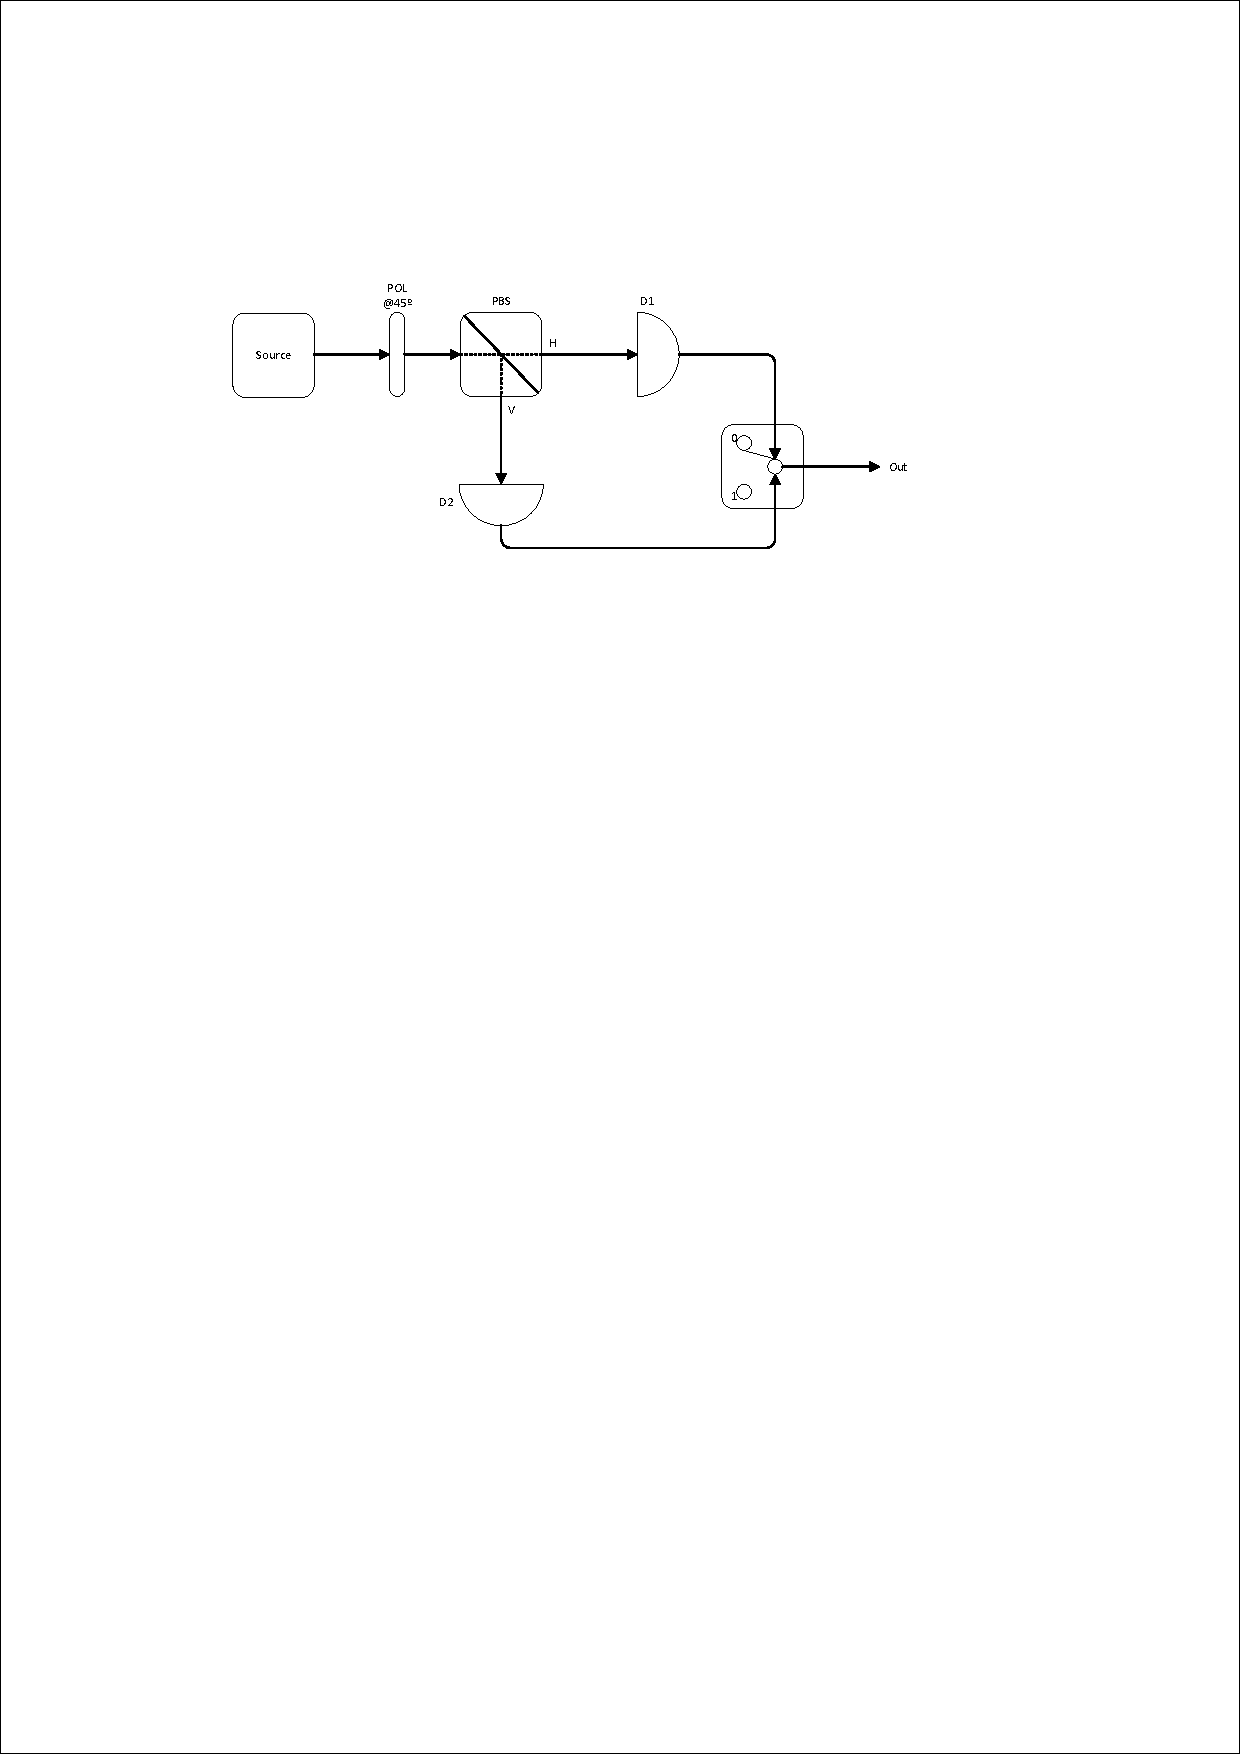
\includegraphics[clip, trim=3cm 20cm 5cm 5cm, width=1.00\textwidth]{./sdf/quantum_random_number_generator/figures_raw/Random_Number_Generator.pdf}
    \caption{Source of randomness with a polarization beam splitter PBS where the incoming light is polarized with POL at $45^{\circ}$ with respect to the PBS.}\label{qrng}
\end{figure}

The principle of operation of the random generator is shown in figure \ref{qrng}. Each individual photon coming from the source is polarized at $45^\circ$ and has equal probability of found in the horizontal polarization (H) or in the vertical polarization (V) output of the PBS. However, quantum theory estimates for both cases the individual choices are truly random and independent one from each other. This way, the detection of the photons in each output of the polarization beam splitter is done with single photon detectors and combining the detection pulse in a switch, which has two possible states: '0' or '1'. When the detector \textbf{D1} fires, the switch is flipped to state '0' and does not mode until a detection event in detector \textbf{B2} occurs and it does not move until a detection occurs in detector \textbf{D1}. In the case of some detections occur in a row in the same detector, only the first detection clicks and the following detections leave the switch unaltered. 

\subsection{Simulation Analysis}



\subsection{Open Issues}



\cleardoublepage
